\section{Dữ liệu 2}
Bộ dữ liệu ghi lại lịch sử về những ngôi nhà được bán từ 5/2014 đến 5/2015 ở quận King, bang Washington, Hoa Kỳ. Bộ dữ liệu bao gồm 21613 quan trắc, gồm 21 biến.
\subsection*{Tìm hiểu dữ liệu}
%một vài quan trắc đầu tiên, bảng correlation, quan sát phân bố biến Y
\begin{figure}[h!]
\centering
\subfloat[Một số quan trắc đầu tiên]
{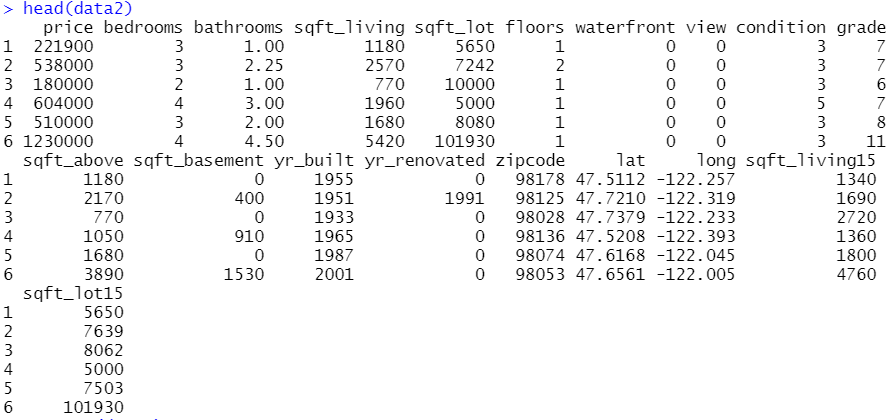
\includegraphics[width=0.7\linewidth]{../Photo Of Result/B2_headdata}}\\
\subfloat[Hệ số tương quan giữa các biến]	{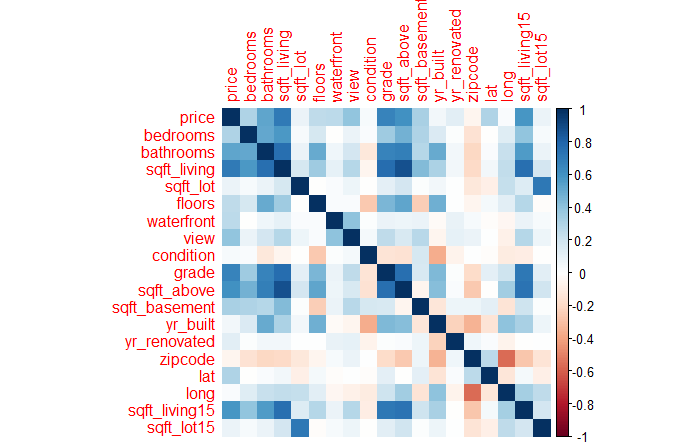
\includegraphics[width=.5\linewidth]{../Photo Of Result/B2_corr}}\hfill
\subfloat[Phân bố của biến phụ thuộc]
{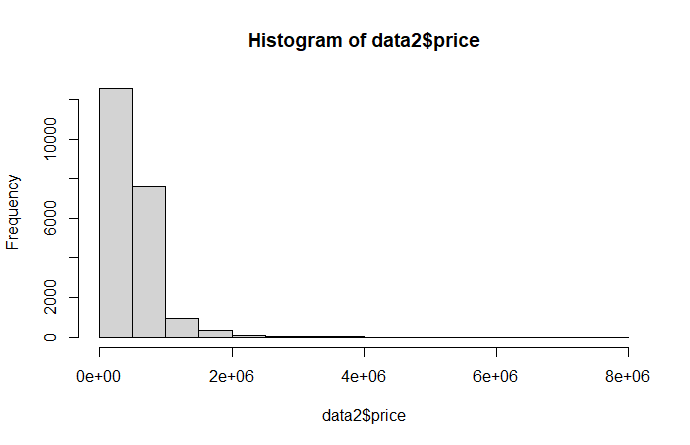
\includegraphics[width=.5\linewidth]{../Photo Of Result/B2_histPrice}}\hfill
\caption{Một số quan sát ban đầu của bộ dữ liệu}
\end{figure}

Bộ dữ liệu cung cấp gồm 21 biến, trong đó biến \textbf{id} và \textbf{date} sẽ được loại bỏ khỏi dữ~liệu trước khi tiến hành phân tích, vì nhóm em nghĩ các biến này chỉ để ghi lại chỉ số và thời gian mua bán, không có ý nghĩa thống kê. 

\subsection*{Phân tích, chọn mô hình}
%mô hình ban đầu (Đầy đủ biến, chưa chuẩn hóa), mô hình sau khi chọn biến bằng các tiêu chuẩn ..., mô hình cuối cùng (nếu có chuẩn hóa dữ liệu)

%đưa ra kết quả R của mỗi mô hình, giải thích vì sao chọn mô hình cuối cùng, phân tích các kết quả từ plot xem mô hình có đảm bảo các giả thiết hay không (kỳ vọng = 0, phân phối chuẩn, phương sai không đổi, có mối quan hệ tuyến tính, không có đa cộng tuyến)
\begin{figure}[h!]
	\centering
	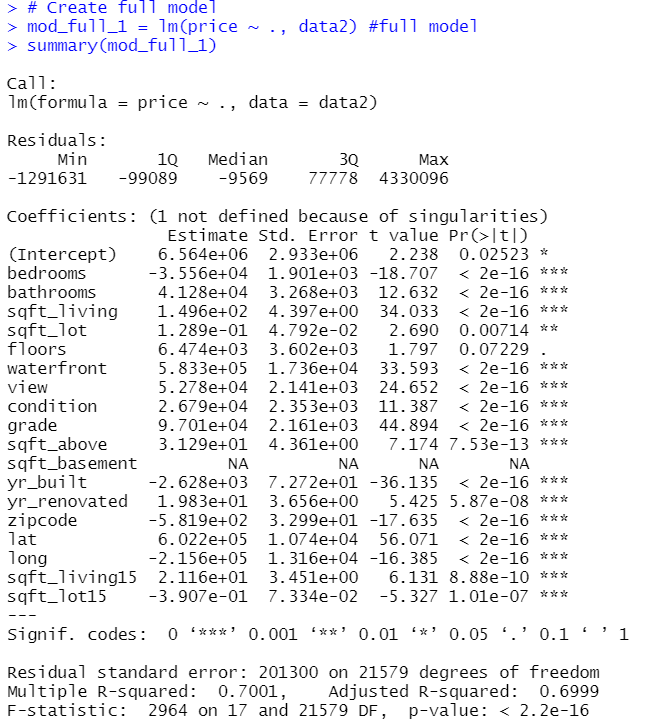
\includegraphics[width=0.7\linewidth]{../Photo Of Result/B2_originalmodel_R}
	\caption{Mô hình hồi quy đầy đủ ban đầu}
	\label{B2_full}
\end{figure}
$*$ \textbf{Phương pháp chọn: Stepwise - lùi; tiêu chuẩn chọn: BIC}.

Bộ dữ liệu (sau khi loại bỏ id và date) có 18 biến giải thích, do đó nhóm em chọn phương pháp lùi (\textbf{stepwise - backward}) cho bộ dữ liệu này. Trong mô hình hồi quy đầy đủ (Hình \ref{B2_full}), đa số các biến giải thích đều có ý nghĩa thống kê, do đó tiến hành phương~pháp lùi (loại biến dần dần) sẽ tiết kiệm thời gian hơn so với các phương pháp còn lại.

\begin{figure}[h!]
	\centering
	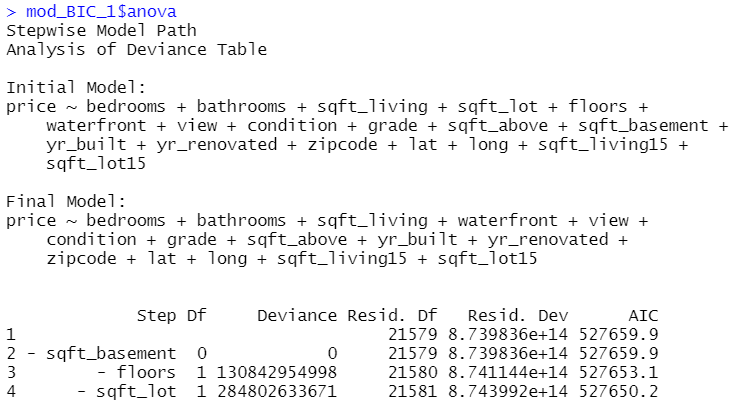
\includegraphics[width=0.7\linewidth]{../Photo Of Result/B2_BIC}
	\caption{Mô hình khi chọn bằng tiêu chuẩn BIC}
	\label{B2_BIC}
\end{figure}



\subsection*{Kết luận}
%Nhận xét các biến ảnh hưởng đến biến Y từ mô hình cuối cùng, ý nghĩa của mô hình đã chọn